\subsection{Bericht integriteit en digitale handtekening}
\subsubsection{Cryptografische hash functies}

Een hashfunctie neemt een invoer, m, en berekent een vaste string grootte H(m). Een cryptografische hash functie is noodzakelijk om de volgende functionaliteit te hebben:
\begin{itemize}
\item Het is rekenkundig onmogelijk om twee verschillende berichten x en y te vinden zodat H(x) = H(y).
\end{itemize}

\noindent Dit betekent dat het rekenkundig onmogelijk is voor een indringer om een bericht te vervangen met een ander bericht die beschermd is door de hash functie. Dat is als (m, H(m)) het bericht en hash zijn van het bericht die gecreëerd is door de zender. Dan kan de indringer de inhoud van een ander bericht y niet vervalsen, dat dezelfde hash waarde heeft als het originele bericht.

\noindent Een \textcolor{red}{\textbf{simple checksum}} zoals de Internet checksum, zou een \textbf{zwakke} cryptografische hash functie zijn. Het is hier mogelijk om \textbf{dezelfde} checksum te bekomen met een verschillend bericht. Dit komt onze voorwaarde niet na. We gaan een andere krachtigere functie nodig hebben.

\subsubsubsection{Hashfunctie algoritmes}

\bi
\itf MD5 hashfunctie is wereldwijd gebruikt
    \bi
    \itf Berekent 128-bit berichtsamenvatting (= message digest) in 4-stappen process.
    \itf Arbitrary 128-bit string x, appears difficult to construct msg m whose MD5 hash is equal to x
    \ei

\itf SHA 1 = Secure Hash Algoritme = wordt ook gebruikt
    \bi
    \itf US Standard
    \itf 160-bit berichtsamenvatting (= message digest)
    \ei
\ei
De MD5 hash algoritme berekent een 128 bit hash in een vier-stappen proces bestaande uit een aanvullende-stap (aanvullen van nullen zodat de lengte van het bericht aan bepaalde condities voldoet), een toevoegingsstap (toevoeging van een 64 bit representatie van de lengte van het bericht), een initialisatie van een accumulator, en een laatste lus-stap waarin het bericht van 16-woorden blokken verwerkt zijn in vier rondes.

\begin{figure}[h]
    \centering
    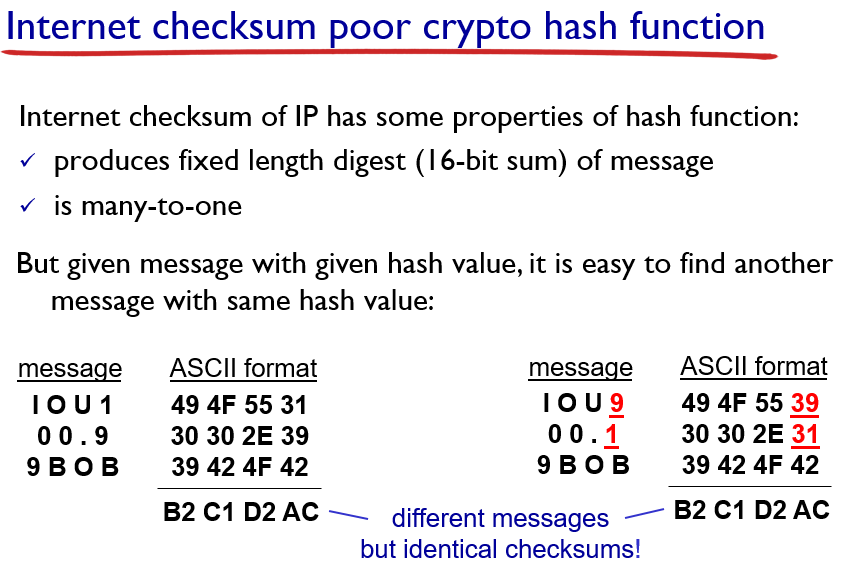
\includegraphics[width=4in]{./img/imghfdst8/hfdst8puntje9.png}
    \caption{internet checksum  }      
    \label{fig:internet checksum }
\end{figure}



\subsubsection{Bericht authenticatie code}

Laten we een eerste gooi doen naar hoe we bericht integriteit kunnen uitvoeren:
\begin{enumerate}
    \item De zender maakt een bericht m en berekent de hash H(m).
     \item De zender maakt H(m) vast aan het bericht door een uitgebreid bericht te maken (m, H(m)), en verzend deze naar de ontvanger.
 \item De ontvanger krijgt het uitgebreide bericht (m, h) en berekent H(m). Als H(m) = h, kan de ontvanger concluderen dat alles inorde is.
\end{enumerate}
Deze benadering is uiteraard gebrekkig. Een indringer kan een vals bericht m´ maken waarin deze zegt dat hij de zender is, H(m´) berekent en naar de ontvanger stuurt. Wanneer de ontvanger het bericht krijgt, gaat alles in orde zijn en zal de ontvanger niets vermoeden.

\noindent Om bericht integriteit uit te voeren, naast het gebruik van cryptografische hash functies, hebben de zender en ontvanger een gedeelde geheime s nodig. Dit gedeeld geheim, is niets meer dan een string van bits die de authenticatie sleutel wordt genoemd. Het gebruik van dit gedeelde geheim, kan bericht integriteit uitgevoerd worden als volgt:
\begin{enumerate}
    \item De verzender maakt een bericht m en voegt s met m om m + s te maken, en berekent de hash H(m + s). Dit wordt de \textcolor{red}{\textbf{\acrfull{mac}}} genoemd.
    \item De verzender voegt de MAC toe aan het bericht m door een uitgebreid bericht te maken (m, H(m + s)), en verzend deze naar de ontvanger.
    \item De ontvanger krijgt het uitgebreide bericht (m, h) and al wetend van s, berekent hij de MAC H(m + s). Als H(m + s) = h kan de ontvanger concluderen dat alles in orde is.
\end{enumerate}
Een leuk kenmerk van een MAC is dat er \textbf{geen nood} is aan encryptie algoritme. Door gebruik te maken van MAC, kunnen de entiteiten de berichten authenticeren die ze naar elkaar sturen zonder het integreren van een complexe encryptie algoritme.
Er blijft nochtans een belangrijke gebrekking. Hoe kunnen we de gedeelde authenticatie sleutel verdelen naar de communicerende entiteiten?



\subsubsection{Digitale handtekening}

Dit is een cryptografische techniek vergelijkend met een handtekening zetten.
\bi
\itf De afzender (Bob) signeert het document digital, waarmee hij aantoont dat hij de eigenaarn en maker van het document is. 
\itf \textcolor{red}{\textbf{Verifieerbaar en niet hermaakbaar:}} de ontvanger (Alice) moet kunnen aantonen aan anderen dat Bob en niemand anders (inclusief Alice) het document gesigneerd heeft.
\ei

\noindent Een simpele digitale handtekening zetten voor het bericht \textbf{m}:

\noindent $\Rightarrow$ Bob tekent \textbf{m} door het encrypteren met zijn private sleutel $K^-_B$ waarmee hij het gesigneerde bericht aanmaakt, $K^-_B (m)$


\begin{figure}[h]
    \centering
    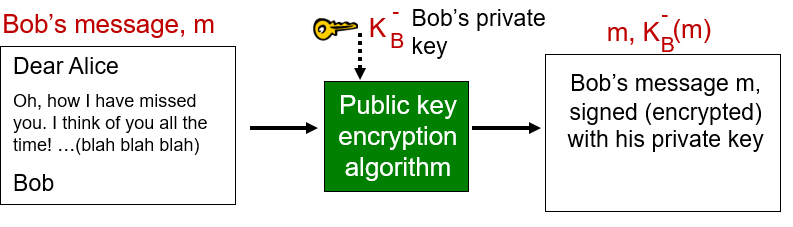
\includegraphics[width=7in]{./img/imghfdst8/hfdst8puntje7.png}
    \caption{Digitale handtekening zetten }      
    \label{fig:Digitale handtekening zetten  }
\end{figure}

\noindent $\Rightarrow$ suppose Alice receives msg m, with signature: m,  $K^-_B (m)$

\noindent $\Rightarrow$ Alice verifies m signed by Bob by applying Bob’s public key  $K^+_B (m)$ to  $K^-_B (m)$ then checks  $K^+_B (K^-_B (m)) = m $.

\noindent $\Rightarrow$ If $K^+_B (K^-_B (m)) = m $ , whoever signed m must have used Bob’s private key.

\noindent Alice verifieert dus dat:

\bi
\itf Bob m heeft ondertekend
\itf niemand anders m heeft ondertekend
\itf Bob m heeft ondertekent en niet m'
\ei

\noindent De verzender kan overwegen om een MAC toe te voegen als ondertekening, waar de MAC is gemaakt door het toevoegen van zijn sleutel (die uniek is voor hem) aan het bericht, en dan de hash te nemen. Maar voordat de ontvanger de ondertekening kan verifiëren, heeft ze ook een kopie nodig van de sleutel. In dit geval zou de sleutel niet meer uniek zijn voor enkel de verzender. \textbf{MAC’s zijn dus geen oplossing.}

\noindent Dit kan opgelost worden met de publieke en privé sleutels van de zender. Want deze zijn uniek voor hem. Bob wilt een een document m digitaal handtekenen. Bob maakt gebruik van zijn privé sleutel $K^-$ om $K^-$(m) te berekenen.

\noindent Voldoet de digitale handtekening $K^-$(m) aan de vereisten van verifieerbaar en niet vervalsbaar te zijn? Wanneer we de publieke sleutel van Bob erbij pakken en toevoegen bij de digitale handtekening $K^-$(m), geassocieerd met het document m. Als $K^+$($K^-$(m)) berekent komt men m uit. 

\noindent Volgende argumenten wijzen dat enkel Bob het document heeft kunnen tekenen:
\begin{itemize}
\item Wie ook het bericht heeft ondertekend, had de privé sleutel $K^-$ om zo de handtekening $K^- (m)$ te berekenen, zodat $K^+(K^- (m)) = m$.
\item De enige persoon die de privé sleutel kende is Bob.
\end{itemize}
\noindent Het is ook belangrijk op te merken dat het originele document m, nooit is aangepast naar een andere vorm m´. De handtekening die Bob heeft gemaakt voor m, gaat niet geldig zijn voor m´. We zien dus dat digitale handtekening ook zorgen voor bericht integriteit.
Een zorg bij het tekenen van data door encryptie is dat encryptie en decryptie zijn computationeel duur. Een efficiëntere benadering is om hash functies te introduceren in de digitale handtekening. Bob tekent de hash van een bericht, in plaats van het bericht zelf, dat is $K^{-}(H(m))$. Sinds H(m) algemeen veel kleiner is, wordt de computationele inspanning om een digitale handtekening te maken aanzienlijk gereduceerd.

\noindent Bob verstuurt een bericht naar Alice. Bob zet zijn bericht in een hash functie en handtekend deze hash daarna digitaal met zijn privé sleutel. Het originele bericht samen met de digitale gehandtekend bericht wordt verzonden naar Alice. Alice voegt de publieke sleutel toe aan het bericht om zo het hash resultaat de krijgen. Alice voert de hash functie uit op de cleartext om een tweede hash resultaat te bekomen. Als deze twee gelijk zijn, kan Alice zeker zijn van de integriteit en auteur van het bericht.

\noindent Een digitale handtekening is dus een “zwaardere” techniek, omdat het een onderliggende \textbf{Public Key Infrastructure (PKI)} met \textbf{ certificaten autoriteiten (\acrshort{ca})} nodig heeft.

\subsubsubsection{CA = certificatie Autoriteit}

\noindent $\Rightarrow$ Deze bindt een publieke sleutel aan een particuliere Entiteit, E.

\noindent $\Rightarrow$ Authenticeert de echtheid van identiteiten en geeft certificaten uit.

\noindent E(persoon of router) registreert zijn publieke sleutel bij een CA.

\noindent Een CA heeft als taken:
\bi
\itf Een CA garandeert dat een entiteit wel degelijk de entiteit is die ze beweert te zijn.
\itf De CA creeërt een certificaat waarmee de openbare sleutel van de entiteit gekoppeld wordt aan de identiteit van de entiteit (E).
    \bi
    \itf het certificaat bevat de openbare sleutel en unieke informatieve over de eigenaar van de openbare sleutel (vb de werkelijke naam of een IP-adres). Dit certificaat wordt digitaal ondertekend door de CA. 
    \ei
\ei

\subsubsubsection{Publieke sleutel certificatie}

Een belangrijke toepassing bij digitale handtekeningen is de \textbf{Publieke Sleutel Certificatie}. Zij certificeren dat een publieke sleutel bij een specifieke entiteit hoort.

\noindent Een CA heeft volgende functies:
\begin{itemize}
\item Een CA verifieert dat een entiteit is wie hij zegt dat hij is. Als het gaat om een CA, moet men erop vertrouwen dat de CA een voldoende strenge identiteitscontrole hebben uitgevoerd. Je kan enkel de identiteit geassocieerd met de publieke sleutel vertrouwen voorzover je de CA kan vertrouwen in zijn identiteit validatie technieken. (Web of trust)
\item Eenmaal dat de CA de identiteit van een entiteit verifieert, maakt de CA een certificaat die gebonden wordt de publieke sleutel van de entiteit aan de identiteit. Het certificaat bevat de publieke sleutel en globaal unieke identificerende eigenschappen over de eigenaar (zoals menselijk naam, IP adres, ...). Het certificaat is digitaal getekend door de CA.
\end{itemize}

\begin{figure}[h]
    \centering
    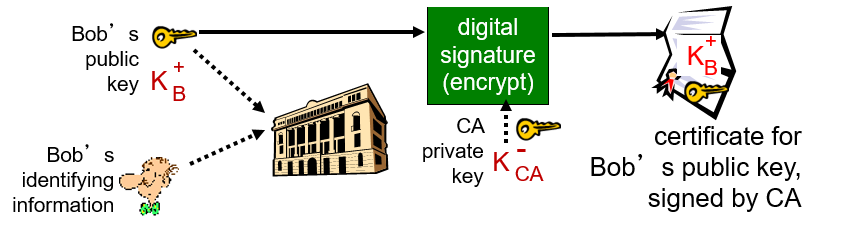
\includegraphics[width=4in]{./img/imghfdst8/hfdst8puntje11.png}
    \caption{Schema aanvraag signing certificaat  }      
    \label{fig:Schema aanvraag signing certificaat }
\end{figure}

\noindent Wanneer Alice de publieke sleutel van Bob wilt:

\bi
\itf krijgt ze Bob’s certificaat)
\itf past ze de publieke sleutel van de CA toe op Bob’s certificaat om te verifiëren
\itf krijgt ze Bob’s publieke sleutel. 
\ei

\begin{figure}[h]
    \centering
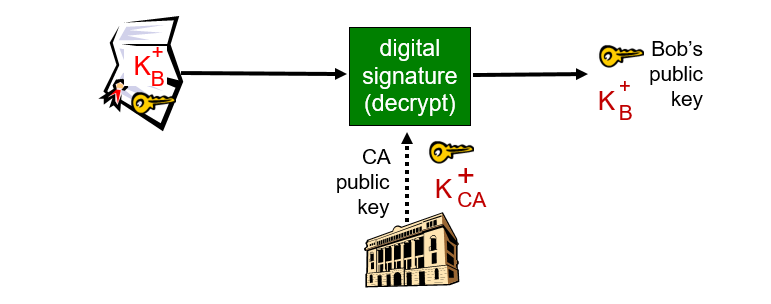
\includegraphics[width=4in]{./img/imghfdst8/hfdst8puntje12.png}
\caption{CA ondertekent certificaat }      
    \label{fig:CA ondertekent certificaat }
\end{figure}